\chapter{Pressupost aproximat del prototip}
\label{chap:Pressupost del prototip}

%Introducció
Per falta de coneixements no s'ha pogut realitzar un prototip real funcional, el qual es pugui contrastar d'una forma objectiva i real amb \newline l'orionBMS, que era el que volíem mostrar. Tot i així si que podem fer una comparació a nivell econòmic per tal de veure per quin cost sortiria aquest BMS. S'han realitzat les recerques de components vàlids per a la implementació d'aquest prototip i s'han posat a més a més, els costos aproximats de la fabricació de la PCB i del muntatge mecànic i de soldadura de la PCB. Aquests preus de muntatge i fabricació estan contrastats amb els costos aproximats de l'empresa on hi treballo.

\begin{figure}[H]
	\centering
    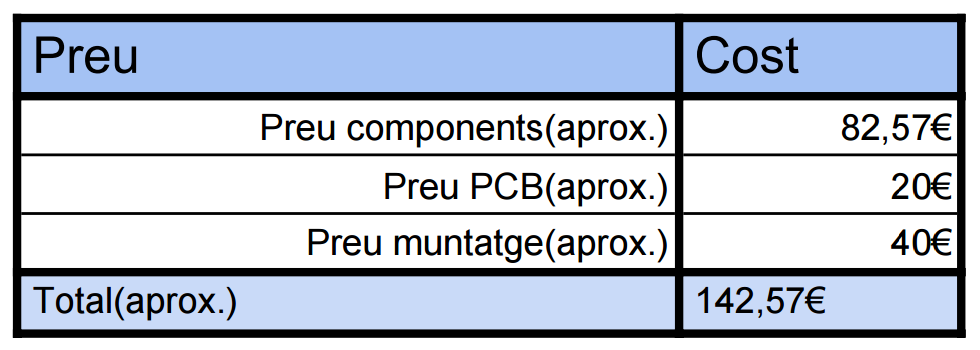
\includegraphics[width=\textwidth, height=5cm] {Pressupost/costBMS.png}
\end{figure}

La llista de components queda mostrada a la següent taula:

\newpage

\begin{figure}[H]
	\centering
    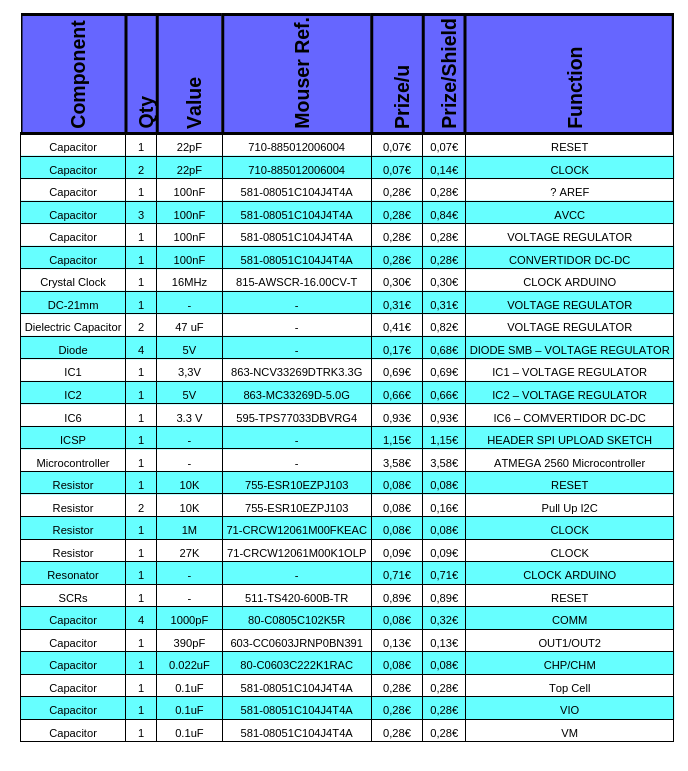
\includegraphics[width=\textwidth, height=\textheight] {Pressupost/componentsp1.png}
\end{figure}

\begin{figure}[H]
	\centering
    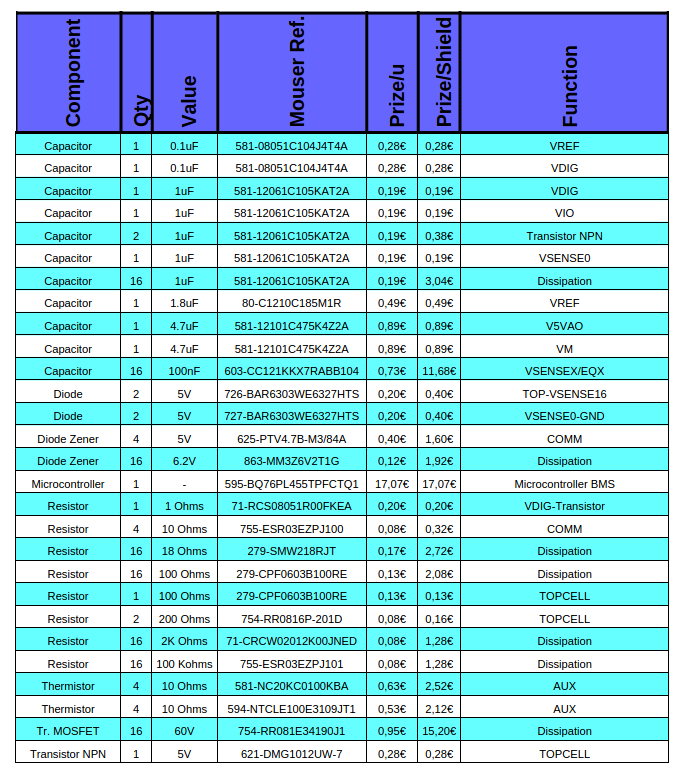
\includegraphics[width=\textwidth, height=\textheight] {Pressupost/componentsp2.png}
\end{figure}